\title{ParProg CheatSheet}
\author{dthoma, lroellin}
\date{August 2017}

\documentclass[a4paper, fontsize=6pt]{scrartcl}
\usepackage{multicol}
\usepackage{calc}
\usepackage{ifthen}
\usepackage[landscape]{geometry}
\usepackage{hyperref}
\usepackage{graphicx}
\usepackage{mathtools}
\usepackage{gensymb}
\usepackage{minted}
\usemintedstyle{bw}
\usepackage{ragged2e} 
\usepackage[T1]{fontenc}
\usepackage[utf8]{inputenc}
\usepackage{amsbsy}
\usepackage{amsfonts}
\usepackage{varwidth,pst-tree,pst-eps}
\usepackage{comment}
\usepackage{xcolor}

\usepackage{fontspec}

\setromanfont[
Path=fonts/Roboto/,
BoldFont=Roboto-Bold.ttf,
ItalicFont=Roboto-Italic.ttf,
BoldItalicFont=Roboto-BoldItalic.ttf
]{Roboto-Regular.ttf}
\setmonofont[
Path=fonts/Hack/,
BoldFont=Hack-Bold.ttf,
ItalicFont=Hack-Italic.ttf,
BoldItalicFont=Hack-BoldItalic.ttf
]{Hack-Regular.ttf}

%German-specific commands
%--------------------------------------
\usepackage[german]{babel}
%--------------------------------------

\graphicspath{ {images/} }


% This sets page margins to .5 inch if using letter paper, and to 1cm
% if using A4 paper. (This probably isn't strictly necessary.)
% If using another size paper, use default 1cm margins.
\geometry{top=0.5cm,left=0.5cm,right=0.5cm,bottom=0.5cm}

% Turn off header and footer
\pagestyle{empty}
 

% Redefine section commands to use less space
\makeatletter
\renewcommand{\section}{\@startsection{section}{1}{0mm}%
    {-1ex plus -.5ex minus -.2ex}%
    {0.5ex plus .2ex}%x
    {\normalfont\large\bfseries}}
    
\renewcommand{\subsection}{\@startsection{subsection}{2}{0mm}%
    {-1explus -.5ex minus -.2ex}%
    {0.5ex plus .2ex}%
    {\normalfont\normalsize\bfseries}}
    
\renewcommand{\subsubsection}{\@startsection{subsubsection}{3}{0mm}%
    {-1ex plus -.5ex minus -.2ex}%
    {1ex plus .2ex}%
    {\normalfont\small\bfseries}}
    
\makeatother

% Define BibTeX command
\def\BibTeX{{\rm B\kern-.05em{\sc i\kern-.025em b}\kern-.08em
    T\kern-.1667em\lower.7ex\hbox{E}\kern-.125emX}}

% Don't print section numbers
%\setcounter{secnumdepth}{0}


\setlength{\parindent}{0pt}
\setlength{\parskip}{0pt plus 0.5ex}


% -----------------------------------------------------------------------

\begin{document}

\footnotesize
\begin{multicols*}{5}


% multicol parameters
% These lengths are set only within the two main columns
%\setlength{\columnseprule}{0.25pt}
\setlength{\premulticols}{1pt}
\setlength{\postmulticols}{1pt}
\setlength{\multicolsep}{1pt}
\setlength{\columnsep}{2pt}

Original von felix.morgner, bearbeitet durch lroellin und dthoma.

\section{Threads}

Für den Start des Threads muss die Methode \mintinline{java}{start()} aufgerufen werden. Ein Aufruf von \mintinline{java}{run()} würde blockieren.

\begin{minted}{java}
new Thread(() -> {
  try {
    function();
  } catch (InterruptedException e) {
    e.printStackTrace();
  }
});

public class SimpleThread extends Thread {
  @Override
  public void run() {
    function();
  }
}
new SimpleThread('.', 10).start();

public class RThread implements Runnable {
  @Override
  public void run() {
    function();
  }
}
new Thread(new RunnableThread('.', 10));
\end{minted}

Eine vierte Möglichkeit wäre eine anonyme innere Klasse. \\

Eine spezielle Art von Threads sind Daemon Threads (\mintinline{java}{t.setDaemon (true);}). Diese Threads verhindern das Beenden des Programms NICHT. Der Garbage Collector ist ein solcher Thread. Sie brechen beim Beenden der JVM unkontrolliert ab.

\section{Synchronisationsprimitiven}

\subsection{Monitor}
Für einfachen (ineffizienten) gegenseitigen Ausschluss (mutual exclusion) gibt es den \mintinline{java}{synchronized} Schlüssel. Die Synchronisierung mittels \mintinline{java}{synchronized} ist reentrant. Das heisst ein Thread kann mehrere \mintinline{java}{synchronized} Methoden verschachtelt aufrufen.

\begin{minted}{java}
public class MyClass {
  public synchronized void one() {
    dangerous_things(); 
  }

  public synchronized void two() {
    dangerous_things();
  }

  public void partlySync() {
    non_dangerous_things();
    synchronized(this) {
      dangerous_things();
    }
  }

  public synchronized void put(int amount)
  throws InterruptedException {
    while (stock + amount > capacity) {
      wait();
    }

    stock += amount;
    notifyAll();
  }
}
\end{minted}

Mit \mintinline{java}{wait(long timeout)} kann man auch nach einem Timer automatisch geweckt werden.

\subsection{Semaphoren}
Semaphore sind Marken und können auch negativ initialisiert werden. Falls keine Marke frei ist (\texttt{<=0}), blockiert \mintinline{java}{acquire()}.

\begin{minted}{java}
public class Warehouse {
  private final Semaphore upperLimit;
  private final Semaphore lowerLimit;

  public Warehouse(int cap, boolean fair) {
    upperLimit = new Semaphore(cap, fair);
    lowerLimit = new Semaphore(0, fair);
  }

  @Override
  public void put(int amount) 
    throws InterruptedException {
    upperLimit.acquire(amount);
    lowerLimit.release(amount);
  }
}
\end{minted}

\subsection{Locks \& Conditions}
Wichtig: bei \mintinline{java}{await()} wird der Lock zwischenzeitig abgegeben. Er muss auch wieder erlangt werden.

\begin{minted}{java}
public class Warehouse {
  private final Lock monitor;
  private final Condition nonFull;
  private final Condition nonEmpty;
  private final int capacity;
  private int stock = 0;

  public Warehouse(int capacity, boolean fair) {
    monitor = new ReentrantLock(fair);
    nonFull = monitor.newCondition();
    nonEmpty = monitor.newCondition();
    this.capacity = capacity;
  }

  @Override
  public void put(int amount) 
  throws InterruptedException {
    monitor.lock();
    while (stock + amount > capacity) {
      nonFull.await();
    }

    stock += amount;
    nonEmpty.signalAll();
    monitor.unlock();
  }
}
\end{minted}

\subsection{Read-Write Locks}
\begin{minted}{java}
public class UpgradeableReadWriteLock {
  private final ReadWriteLock readWriteLock =
  new ReentrantReadWriteLock();
  private final Lock upgradableReadLock = 
  new ReentrantLock();

  public void readLock() throws InterruptedException {
    readWriteLock.readLock().lock();
  }

  public void readUnlock() {
    readWriteLock.readLock().unlock();
  }

  public void upgradeableReadLock() 
  throws InterruptedException {
    upgradableReadLock.lock();
  }

  public void upgradeableReadUnlock() {
    upgradableReadLock.unlock();
  }

  public void writeLock() 
  throws InterruptedException {
    upgradableReadLock.tryLock();
    readWriteLock.writeLock().lock();
  }

  public void writeUnlock() {
    readWriteLock.writeLock().unlock();
    upgradableReadLock.unlock();
  }
}
\end{minted}

\subsection{CountDownLatch}
Bietet einen ''Einweg-Synchronisationspunkt''. Bei der Initialisierung muss angegeben werden, auf wieviele Threads gewartet werden soll. Kann \textbf{nicht wiederverwendet} werden.

\begin{minted}{java}
public class RaceControl {
  CountDownLatch carsReady = 
    new CountDownLatch(NOF_RACE_CARS);
  CountDownLatch startSignal = 
    new CountDownLatch(1);

  protected void waitForAllToBeReady() 
    throws InterruptedException {
    carsReady.await();
  }

  public void readyToStart() {
    carsReady.countDown();
  }

  protected void giveStartSignal() {
    startSignal.countDown();
  }

  public void waitForStartSignal() 
    throws InterruptedException {
    startSignal.await();
  }
}
\end{minted}

\subsection{CyclicBarrier}
Die Cyclic Barrier startet automatisch sobald \texttt{N} Threads warten:
\begin{minted}{java}
CyclicBarrier raceStart = new CyclicBarrier(N);
raceStart.await();
\end{minted}

Die Barrier kann auch für mehrere Runden eingesetzt werden. Bei einer Exeption z.B. \mintinline{java}{InterruptedException}, sind alle betroffen. \mintinline{java}{getParties()} ermittelt die Anzahl Teilnahmer der Barriere.

\subsubsection{Phaser}
stellt eine verallgemeinerte \mintinline{java}{CyclicBarrier} da, bei der die Anzahl verändert werden kann.

\begin{minted}{java}
// anfangs keine Player
Phaser phaser = new Phaser(0);
phaser.register();
while(isRunning) {
  phaser.arriveAndAwaitAdvance();
  playRound();
}
phaser.arriveAndDeregister();
\end{minted}

\subsection{Exchanger}
Ermöglicht es, zwischen zwei Threads Objekte auszutauschen. \mintinline{java}{exchange(obj1)} wartet, bis der andere Thread auch \mintinline{java}{exchange(obj2)} aufgerufen hat.

\begin{minted}{java}
Exchanger<Integer> exchanger = new Exchanger<>();
int out = exchanger.exchange(in);
\end{minted}

\section{Race Conditions, Deadlocks \& Starvation}
\subsection{Race Conditions}
Werden in Low-Level (Data Race?) und High-Level (Semantic Race) unterteilt. \textbf{Low-Level Races} treten auf wenn unsynchronisiert auf den gleichen Speicher (Variable, Array-Element, ...) zugegriffen wird. \textbf{High-level Races} sind Race-Conditions in der Programmlogik. Sie treten auf, wenn die Critical Sections nicht ausreichend geschützt sind.

Collections aus \mintinline{java}{java.util} sind grundsätzlich nicht threadsafe. Es gibt jedoch threadsafe Collections in \mintinline{java}{java.util.concurrent}.

Auf Synchronisierung kann \textbf{verzichtet} werden, wenn entweder Unveränderlichkeit (z.B. Java \mintinline{java}{final}) oder  veränderliche Objekte in Objekte eingesperrt sind (Object Confinement).

\subsection{Deadlocks}
treten unter folgenden Bedingungen auf: wenn \textit{geschachtelte Locks}, \textit{zyklische Warteabhängigkeiten}, \textit{gegenseitiger Ausschluss} und \textit{kein Timeout} gemeinsam vorkommen.

Sie lassen sich durch Einführung einer \textit{linearen Sperrordnung} oder \textit{grobgranulare Sperrung} lösen.

Live-Locks sind Deadlocks, bei denen permanent CPU verbraucht wird.

\subsection{Starvation}
tritt auf, wenn einem Thread immer wieder die Möglichkeit zu arbeiten weggeschnappt wird. Dies lässt sich durch faire Synchronisationsprimitiven lösen.

\section{Thread Pools}
besitzen eine \textit{Task Queue}, in welche Tasks eingereiht werden; von dort werden sie dann von einem \mintinline{java}{Worker Thread} herausgenommen und bearbeitet. Worker Threads sind Daemon-Threads. Seit Java 7/8 gibt es den \mintinline{java}{ForkJoinPool}. Beim Beenden des Programms werden die Worker-Threads einfach terminiert, weil sie Deamon-Threads sind.

\begin{minted}{java}
ForkJoinPool tp = new ForkJoinPool();
Future<Integer> l = tp.submit(() -> count(lPart));
Future<Integer> r = tp.submit(() -> count(rPart));
int result = l.get() + r.get();
\end{minted}

\subsection{Recursive Action}
\begin{minted}{java}
public class ParalellQS extends RecursiveAction {
  @Override
  protected void compute() {
    List<ParalellQS> tasks = new LinkedList<>();
    if (j > left) {
      tasks.add(new ParalellQS(array, left, j));
    }
    invokeAll(subtasks);
  }
}

class CountTask extends RecursiveTask<Integer> {
    protected Integer compute() {
        CountTask left = new CountTask(leftPart);
        CountTask right = new CountTask(rightPart);
        left.fork(); right.fork();
        return right.join() + left.join();
    }
}

pool.invoke(new MergeSortTask(array, 0, array.length));
// oder
new MergeSortTask(array, 0, array.length).invoke();
\end{minted}

Man kann auch den Pool auswählen. Entweder einen eigenen ForkJoinPool, oder den \textit{Common Pool}. Diesen teilt man mit dem Rest der JVM, er wird noch nicht empfohlen. Direkt auf dem Common Pool starten: \mintinline{c}{new CountTask(args).invoke();}

\subsection{Work Stealing}
Der Pool hat eine globale Task Queue, die Worker Threads eine lokale Queue damit sie nicht nach jedem Task die globale sperren müssen, um neue zu holen. Wenn ein Worker Thread seine Queue abgearbeitet hat, und er keine mehr in der globalen findet, kann er auch Tasks aus der Queue eines anderen Worker Threads holen.

\section{Future}
\mintinline{java}{CompletableFuture}s laufen automatisch auf dem Common Pool.

\begin{minted}{java}
public CompletableFuture<String> asyncDl(String l) {
  return CompletableFuture.supplyAsync(
    () -> downloadUrl(l));
}

CompletableFuture<String> download = 
downloader.asyncDownloadUrl(link);
download.thenAccept(
  result -> System.out.println(result));
System.out.println(download.get());
\end{minted}

\mintinline{java}{thenApply()} für Funktion mit Rückgabe, \mintinline{java}{thenAccept()} für Handler ohne Rückgabe (typischerweise am Ende). \mintinline{java}{.allOf(fut1, fut2).thenAccept(...)} wenn alle fertig sind, \mintinline{java}{.anyOf(fut1, fut2).thenAccept(...)} wenn einer davon fertig ist.

\section{.NET und TPL}

\subsection{TPL (Task Parallel Library)}
ist ein Work Stealing Thread Pool. Die TPL erkennt geschachtelte Tasks automatisch. Die TPL erzeugt selber neue Tasks, wenn sie merkt dass der Durchsatz sinkt (Hill-Climbing Algorithmus). Somit können Deadlocks bei Task-Abhängigkeiten verhindert werden (ausser man setzt die maximale Anzahl mit \mintinline{csharp}{ThreadPool.SetMaxThreads(n)}).

\begin{minted}{csharp}
Task<int> task = Task.Run(() => {
  return 42;
});
task.Result; // blockiert
// task.Wait ohne <> Rückgabewert

Task.Run(() => {
  Task<int> left = Task.Run(
    () => Count(leftPart));
  Task<int> right = Task.Run(
    () => Count(rightPart));
  int result = left.Result + right.Result
});
task.Result; // blockiert
// task.Wait ohne <> Rückgabewert
\end{minted}

\subsection{Einfache Parallelität}
\begin{minted}{csharp}
Parallel.For(0, array.Length,
  i => DoComputation(array[i])
);

Parallel.Invoke(
    () => QuickSort(array, left, right),
    () => QuickSort(array, left, right)
);

bookCollection.
  Where(book => book.Title.Contains("Concurrency")).
  Select(book => book.ISBN)
  
List<Task> tasks = new List<Task>();
foreach(string link in links) {
    tasks.Add(Task.Run(() => DownloadWebsite(link)));
}
Task.WhenAll(tasks).ContinueWith(
  pd => Console.WriteLine("{t} ms")).Wait();
\end{minted}

\subsection{async/await}
erlauben das teil-asynchrone Ausführen von Funktionen. Der Compiler zerlegt die \mintinline{csharp}{async}-Funktion in zwei Hälften: bis zum ersten  \mintinline{csharp}{await} wird die Funktion vom Caller synchron ausgeführt. Der Rest wird auf einem TPL-Thread erledigt.

\mintinline{csharp}{await} darf nur in \mintinline{csharp}{async}-Funktionen vorkommen; \mintinline{csharp}{async}-Funktionen müssen ein \mintinline{csharp}{await} enthalten.

Hinter den Kulissen baut \mintinline{csharp}{await} die nachfolgenden Aufrufe in eine Continuation. Ist der Aufrufer ein UI-Thread, dann wird die Continuation auf den UI-Thread dispatched, andernfalls auf einen normalen TPL-Threads.

Achtung: \mintinline{java}{async/await} kann zu einem Threadwechsel innerhalb eines Funktionsaufrufs führen!

\section{Java UI}

\begin{minted}{java}
public ComputerGUI(Computer computer) {
  this.computer = computer;
  computer.addObserver(this);
}

ForkJoinPool tp = new ForkJoinPool();
startButton.addActionListener(event -> {
  tp.submit(() -> {
    String r = computer.calc();
    SwingUtilities.invokeLater({
      () -> resultLabel.setText("Result: " + r));
      // kann auch rekursiv nochmal tp.submit(...)
      // und auch dort nochmal .invokeLater(...)
  })
});
public void update(Observable o, Object arg) {
    SwingUtilities.invokeLater(
      () -> statusLabel.setText(computer.getStatus()));
}
\end{minted}

\section{Memory Models}
\subsection{Java}

\subsubsection{Atomicity}
Zugriff auf Variable (Lesen/Schreiben) ist atomar für primitive Datentypen bis 32 Bit, Objekt referenzen, \mintinline{java}{volatile long} und \mintinline{java}{volatile double}.

\subsubsection{Visibility}
Die Sichtbarkeit ist garantiert bei Locks Release \& Acquire,  \mintinline{java}{volatile}-Variablen (für while true), \mintinline{java}{final}-Variablen nach dem Ende des Konstruktors, Thread-Start/Join und Task-Start/Ende.

\subsubsection{Ordering}
\mintinline{java}{volatile} garantiert, dass kein Reordering über einen Zugriff (r/w) auf diese Variable hinaus statt findet. Das Ordering vor und nach \mintinline{java}{volatile} folgt innerhalb des Threads der \textit{As-if-Serial} Semantik. Das heisst, der Compiler darf optimieren falls die Semantik innerhalb des Threads gleich bleibt.

Zwischen Threads ist Ordering nur bei \mintinline{java}{volatile}-Variablen und bei Synchronisationsbefehlen garantiert. \mintinline{java}{volatile}-Variablen führen nicht zu Locking.

\subsection{Atomare Operationen in Java}
Atomare Operationen garantieren Ordering und Visibility. Beispiele sind \mintinline{java}{getandSet(newVal)}, \mintinline{java}{getAndAdd(delta)} und \mintinline{java}{updateAndGet(lambda)}.

Mit \mintinline{java}{boolean compareAndSet(old, new)} kann man atomar auf einen Wert prüfen, und falls dieser stimmt, einen neuen Wert setzen. Der Rückgabewert zeigt ob die Ersetzung stattgefunden hat.

Achtung, bei diesem Beispiel kann man in das ABA-Problem laufen. Idee: berechne etwas mit dem alten Wert, und schreibe das Resultat, falls sich das Objekt nicht verändert hat.
\begin{minted}{java}
private AtomicInteger balance = new AtomicInteger(0);
balance.addAndGet(amount);
do{
  oldBalance = balance.get();
  newBalance = oldBalance - amount;
   if (amount > oldBalance) {
    return false;
   }
  } while (!balance.compareAndSet(oldBalance, newBalance));

do {
    oldV = var.get();
    newV = calcChanges(oldV);
} while (!var.compareAndSet(oldV, newV)
\end{minted}

Es gibt neben AtomicInteger (-Long, -Boolean, ...) für primitive Typen auch AtomicReference<T> für Referenzen.

\subsection{ABA-Problem}
bei unserem Beispiel kann es sein, dass man erst den Wert \mintinline{java}{A} liest, sich dann an die Arbeit macht und schliesslich wieder den Wert \mintinline{java}{A} liest und denkt, es habe sich nichts geändert. In der Zwischenzeit kann aber ein anderer Thread das Objekt angefasst und \mintinline{java}{B} geschrieben haben, was er dann wieder mit \mintinline{java}{A} ersetzt. Davon merken wir nichts, wir können also mit diesem Test nicht davon ausgehen dass das Objekt nicht verändert wurde.

\subsection{.NET}
Unterschied zu Java:
\begin{itemize}
    \item long und double auch mit \mintinline{java}{volatile} NICHT atomar
    \item Visibility implizit durch Ordering gegeben
    \item Ordering: volatile ist nur eine Partial Fence
\end{itemize}

Bei .NET sind also Umordnungen in eine Richtung erlaubt. Will man einen Full Fence, nutzt man \mintinline{java}{Thread.MemoryBarrier();}

Angenommen, wir haben ein \mintinline{java}{volatile int x}. Dann ist das folgende beim \textbf{Lesen} erlaubt:


\includegraphics[scale = 0.1]{VolatileRead}

Und das folgende beim \textbf{Schreiben}

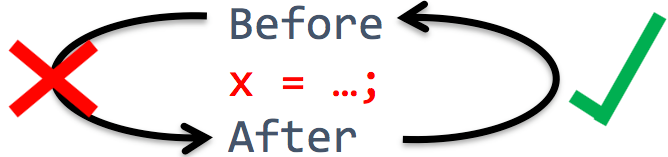
\includegraphics[scale = 0.1]{VolatileWrite}

\section{CUDA}

\subsection{Vokabular}
Eine GPU besteht aus mehreren \textbf{Streaming Multiprocessors (SM)}. Jeder SM besteht aus mehreren \textbf{Streaming Processors (SP)}.

In CUDA ist eine GPU ein \textbf{Grid}, das aus mehreren \textbf{Blöcken} besteht. Jeder Block hat mehrere \textbf{Threads}. Threads werden zu je 32 als \textbf{Warps} zusammengefasst.

\textbf{SIMD} ist die Abkürzung für ''Single Instruction Multiple Data'' und entspricht dem Paradigma der Vektorparallelität. GPUs sind gut für SIMD-Applikationen geeignet, schliesslich führen alle Cores die gleiche Instruktion auf unterschiedlichen Daten aus. 

\subsection{CUDA}

CUDA ist eine Architektur von Nvidia und arbeitet mit sogenannten \textbf{Kernels}, welche auf der GPU laufen. 

Jeder Kernel kann Informationen drüber abrufen, auf welchem Block er läuft (\mintinline{c}{blockIdx.x}), welcher Thread er innerhalb des Blocks ist (\mintinline{c}{threadIdx.x}) und wie gross ein Block ist (\mintinline{c}{blockDim.x}). Es gibt hier immer auch die \mintinline{c}{y-} und \mintinline{c}{z}-Dimension.

Als Programmierer muss man die Datenaufteilung selber modellieren. \textbf{Divergenz} heisst, dass im selben Warp unterschiedliche Pfade vorhanden sind (z.B. if/else). Dies führt zu einem Performance-Problem.

\begin{minted}{c}
__global__
void VectorAddKernel(float *A, float *B,
    float *C, int N) {
    int i = blockIdx.x * blockDim.x
        + threadIdx.x
    // bounds check
    if (i < N) {
        C[i] = A[i] + B[i];
    }
}
\end{minted}

\subsection{CUDA Memory Management}
es gibt die drei Funktionen \mintinline{c}{cudaMalloc}, \mintinline{c}{cudaFree} und \mintinline{c}{CudaMemCpy}.

\subsection{Maximale Thread-Zahl}
Gegeben:
\begin{itemize}
    \item max. Threads per Block: 1024
    \item max. Resident Blocks: 8
    \item max. Resident Threads: 1536
\end{itemize}

Wir wollen einen Vektor mit \textbf{1500} Elementen parallel bearbeiten.

Ausrechnen, dann nach folgender Priorität auswählen:
\begin{enumerate}
    \item Alle Threads müssen in SM passen
    \item am wenigsten unnütze Threads
    \item am meisten Threads per Block
\end{enumerate}

\subsection{CUDA-Grundgerüst}
Ohne Error Handling!

\begin{minted}{c}
void CudaVectorAdd(float* A, float* B, 
  float* C, int N) { 
  size_t size = N * sizeof(float);
  float *d_A, *d_B, *d_C;
  
  cudaMalloc(&d_A, size); // d_B, d_C
  cudaMemcpy(d_A, A, size,
    cudaMemcpyHostToDevice); // d_B
  
  int blockSize = 512;
  int gridSize = (N + blockSize - 1) / blockSize;
  VectorAddKernel<<<gridSize, 
    blockSize>>>(d_A, d_B, d_C, N);
    
  cudaMemcpy(C, d_C, size, 
    cudaMemcpyDeviceToHost); // nur d_C
  cudaFree(d_A); // d_B, d_C
}
\end{minted}

\subsection{Function Keywords}
\begin{itemize}
    \item \mintinline{c}{__global__} läuft auf Device, Aufruf vom Host
    \item \mintinline{c}{__device__} läuft auf Device, Aufruf vom Device
    \item \mintinline{c}{__host__} läuft auf Host, Aufruf vom Host
\end{itemize}

\subsection{Launch Configuration}
muss dynamisch bestimmt werden und sich am Problem und den Fähigkeiten des Devices orientieren (ermitteln mit \mintinline{c}{cudaGetDeviceProperties()}.

Aus Effizienzgründen sollte die Blockgrösse ein Vielfaches von 32 sein. Grosse Blöcke haben den Vorteil, dass die Threads interagieren können.

\subsection{Memory Access} im Device Global Memory ist massiv teurer als Zugriff im Shared Memory (\mintinline{c}{__shared__}). Um Memory \textbf{Coalescing} (mehrere Ladevorgänge zu einem zusammenfassen) zu ermöglichen, sollten Speicherzugriffe möglichst wie folgt aussehen:

\begin{minted}{c}
data[(Ausdruck ohne threadIdx.x) + threadIdx.x]
\end{minted}

Oft kann mit dem Vertauschen von Zeile und Spalte eine Optimierung erreicht werden.

\subsection{Synchronisierung}
kann mittels \mintinline{c}{__syncthreads()} erreicht werden, was alle Threads in einem Block zum Synchronisieren zwingt

\subsection{Effiziente Matrix-Multiplikation}
Ohne Memory Guards!

\begin{minted}{c}
__shared__ float Asub[TILE_SIZE][TILE_SIZE];
__shared__ float Bsub[TILE_SIZE][TILE_SIZE];

int tx = threadIdx.x, ty = threadIdx.y;
int col = blockIdx.x * TILE_SIZE + tx;
int row = blockIdx.y * TILE_SIZE + ty;

for (int tile = 0; tile < nofTiles; tile++) {
  Asub[ty][tx] = A[row * K 
    + tile* TILE_SIZE + tx];
  Bsub[ty][tx] = B[(tile * TILE_SIZE 
    + ty) * M + col];
  __syncthreads();
  for (int ksub = 0; ksub < TILE_SIZE; ksub++) {
    sum += Asub[ty][ksub] * Bsub[ksub][tx];
  }
  __syncthreads();
}
C[row * M + col] = sum;
\end{minted}

\section{Cluster / MPI (Message Passing Interface)}
Cluster weisen spezielle Eigenschaften auf. Shared Memory gibt es nur innerhalb eines Nodes. Sie sind aber mit General Purpose CPUs ausgestattet. Sie tauschen Informationen mit Dateien oder über Sockets aus.

Basiert auf dem Actor- bzw. dem CSP-Modell und ist sehr gut für heterogene Umgebungen geeignet. MPI ist ein Industristandard und ermöglicht \textbf{SPMD} (Single Program Multiple Data), da jeder Node das gleiche Programm mit anderen Daten ausführt.

Ein Task kann mittels \mintinline{bat}{mpiexec -n 100 Program.exe} auf einem HPC Cluster gestartet werden.

\begin{minted}{csharp}
using MPI; 
using System;

class Program {
  public static void Main(string[] args) {
    using (new MPI.Environment(ref args)) {
      int rank = Communicator.world.Rank;
      Console.WriteLine("MPI process {0} ", rank);
      
      if(world.Rank > 0) {
        world.Send(count, 0, 0);
      } else {
        long total = count;
        for (int i = 1; i < world.Size; i++) {
          long value;
          world.Revieve(i, 0, out value);
          total += value;
        } (1000 geschweifte Klammern)
\end{minted}

\mintinline{csharp}{world.Reduce(hits, (a, b) => a + b, 0} kann zum Zusammenfassen der Ergebnisse benutzt werden.

\subsection{Kommunikation} in MPI kann über \mintinline{csharp}{Communicator.world} erfolgen. Um eine Nachricht direkt zu einem Node zu \textbf{senden}, verwendet man \mintinline{csharp}{world.Send(value, receiverRank, messageTag}. Will man entsprechend \textbf{empfangen}, \mintinline{csharp}{world.Receive(senderRank, messageTag, out value}.

Nachrichten an alle können mit \mintinline{csharp}{world.Broadcast(ref value, senderRank} abgesetzt und empfangen werden. Synchronisierung erreicht man mit \mintinline{csharp}{Communicator.world.Barrier()}. Alle Nodes warten dann darauf, dass die Barriere von allen erreicht wird.

Ergebnisse können mit \mintinline{csharp}{AllReduce(T value, OP<T>} (Broadcast) oder \mintinline{csharp}{Reduce(T value, Op<T>, int rank)} (ohne Broadcast) reduziert werden. Es existieren noch weitere Kommunikationsmöglichkeiten wie \mintinline{csharp}{outputArray = AllToAll(inputArray);} \mintinline{csharp}{value = Scatter(array, rank);} \mintinline{csharp}{outputArray = Gather(value, rank)}.

\begin{itemize}
    \item Scatter: einer verteilt verschiedene Werte an alle anderen
    \item Gather: alle senden verschiedenee Werte an einen
\end{itemize}

\section{Reactive Programming}

Asynchrone Datenflüsse führen dazu, dass automatisch parallelisiert werden kann, die Verteilbarkeit gut ist und keine Data-Races, Deadlocks und Starvation auftreten können.

\subsection{.NET PLINQ}
via Extension Methods

\begin{minted}{csharp}
salesEurope.
    Union(salesAsia).
    Union(salesAmerica).
GroupBy(item => item.Article, item => Item.Volume).
Select(category => new {Key = category.Key,
    Value = category.Sum()
}).
Where(category => category.Value >= 1000);
\end{minted}

oder mit der eingebetteten Syntax

\begin{minted}{csharp}
from entry in
    salesEurope.AsParallel().
    Union(salesAsia.AsParallel()).
    Union(salesAmerica.AsParallel()).
group
    entry by entry.Article into category
    let sum = category.Sum(e => e.Volume)
where
    sum >= 1000
select
    new {category.Key, sum};
\end{minted}

Die Reihenfolge der Resultate ist beliebig, fix möglich mit \mintinline{csharp}{AsOrdered()}

\subsection{Rx.NET}
erlaubt das Reagieren auf eine aktive Quelle (\textbf{push}). Das System basiert auf dem Observer-Pattern. Um eine Pipeline zu bauen benötigt man ein Subject, das sowohl Observer als auch Observable ist.

\subsection{Subject}
Ein \mintinline{csharp}{Subject<T>} vereint zwei Interfaces. 1. \mintinline{csharp}{IObservable<T>} mit \mintinline{csharp}{Subscribe(Observer<T>)}. 2. \mintinline{csharp}{IObserver<T>} mit \mintinline{csharp}{OnNext(value: T}), \mintinline{csharp}{OnError(Exception)} und \mintinline{csharp}{OnCompleted()}.

\begin{minted}{csharp}
var subject = new Subject<string>();
subject.Subscribe(Console.WriteLine);

subject.OnNext("A");
subject.OnNext("B");
subject.OnNext("C");

subject.OnCompleted();
\end{minted}

Subjects haben normalerweise kein Gedächtnis, es gibt aber: \mintinline{java}{ReplaySubject}, Observer erhält alle letzten Werte. \mintinline{java}{BehaviorSubject}, schickt letzten Wert und zukünftige. \mintinline{java}{AsyncSubject} schickt letzten Wert bei OnCompleted

Collections können auch zu Observables umgebaut werden:

\begin{minted}{csharp}
var combinedSales = 
    salesEurope.ToObservable().
    Merge(salesAsia.ToObservable()).
    Merge(salesAmerica.ToObservable());

combinedSales.Subscribe(Console.WriteLine);
\end{minted}

\subsection{Ad-hoc Observer Erzeugung}
\begin{minted}{csharp}
subject.Subscribe(
 // OnNext
  value => Console.WriteLine("{0} received", value),
  // OnError
  exception => Console.WriteLine("{0} thrown",
    exception),
  // OnCompleted
  () => Console.WriteLine("completed", value)
);
\end{minted}

\subsection{Concurrency: Scheduler angeben}

\begin{minted}{csharp}
observable.ObserveOn(TaskPoolScheduler.Default).
Subscribe(...)
\end{minted}

\section{Software Transactional Memory (STM)}
Nimmt Ideen aus der Datenbankwelt und versucht damit das Problem des \textbf{Shared Mutable State} ohne Locks und Starvation anzugehen. Es gibt auch Hardware-Implementationen. Meistens wird \textbf{Optimistic Concurrency Control (OCC)} (Rollback bei Konflikt) als Umsetzung verwendet. STM kennt dadurch kein Locking, keine Low-Level Data-Races und keine Deadlocks.

In Java gibt es ScalaSTM, ein deskriptiver Ansatz und somit ein relativ einfaches Programmiermodell. Die Implementierung ist aber sehr komplex und ''teuer''.

\section{Actor Modell}
versucht das Problem zu lösen, dass herkömmliche Sprachen nicht für Nebenläufigkeit entworfen wurden. Kein Shared-Memory und somit keine Low-Level Data-Races.

\subsection{Active Objects}
sind Objekte welche ein Eigenleben führen. Im Actor-Modell gibt es nicht einen ''Chef'', der den Objekten befiehlt was sie tun sollen, sondern die Objekte kommunizieren untereinander.

\subsection{Akka}
ist eine Scala-unterstützte Implementierung des Actor-Modells. Akka Actors verfügen über eine \textbf{Mailbox} um Nachrichten zu empfangen (mittels \mintinline{java}{onReceive} im Actor).

\begin{minted}{csharp}
public class NumberPrinter extends UntypedActor {
    public void onReceive (final Object message) {
        if (message instanceof Integer) {
            System.out.print(message);
        }
        // weitere Message-Arten (bas. auf Klasse)
    }
}
ActorSystem system = 
    ActorSystem.create("System");
ActorRef printer = 
    system.actorOf(Props.create(
        NumberPrinter.class));
    
for (int i = 0; i < 100; i++) {
    printer.tell(i, ActorRef.noSender());
}

system.shutdown();
\end{minted}

\subsection{ActorRef}
speichert eine Referenz auf eine Instanz eines Actors. Dadurch wird verhindert, dass man direkt auf Variablen und Methoden des Actors zugreifen kann. Falls der Actor neu gestartet werden muss, behält er seine Adresse. Man kann die ActorRef in Nachrichten verschicken.

\subsection{Remoting} wird dadurch vereinfacht dass Nachrichten immutable sind. Ein Lookup für einen Actor kann mittels \mintinline{java}{system.actorSelection(urlString)} durchgeführt werden. Das Ergebnis (eine \mintinline{java}{ActorSelection}) kann 0-n Aktoren umfassen und zu einer \mintinline{java}{ActorRef} aufgelöst werden.

\subsection{Messaging} in Akka ist grundsätzlich asynchron. Es kann jedoch mittels Futures synchron auf eine Antwort gewartet werden.

Messages müssen Serializable sein und immutable. Sie dürfen nur final-Felder haben. Sie dürfen nicht über Methoden mit Seiteneffekten verfügen. Collections müssen in \mintinline{java}{Collections.unmodifiableList} verpackt werden.

\begin{minted}{csharp}
Future<Object> result = // immer Object
    Patterns.ask(actorRef, msg, timeout);
result.get();

public class Booking {
    final String name;
    public Booking(String name) {
        this.name = name;
    }
    public String getName() {
        return name;
    }
}
\end{minted}

\subsection{Akka Laufzeitsystem}
setzt typischerweise auf \mintinline{java}{ForkJoinPools} auf, es wird aber aus Effizienzgründen nicht ein Thread pro Actor verwendet.

Synchrones Senden und Empfangen von Nachrichten führt zu Warteabhängigkeiten, was wiederum zu Deadlocks führen kann. Deshalb wird von synchroner Kommunikation abgeraten.

\subsection{Akka Supervision} bezeichnet das Überwachen von Actors durch andere Actors. Eltern überwachen per Default ihre Kinder. Bei einer Exception wird der Supervisor benachrichtigt und muss entscheiden wie es weiter geht. Resume: Kind soll weitermachen. Restart: Kind neustarten. Stop: Kind beenden. Escalate: seinem Supervisor melden, dass er selber nicht weiss wie reagieren

\subsection{System Shutdown}
erfolgt durch das Stoppen der Actors: (alle rekursiv)

Mittels \mintinline{java}{getContext().stop(actorRef)} wird einem Actor mitgeteilt, dass er \textit{nach} Bearbeitung der aktuellen Message anhalten soll. 

Mit \mintinline{java}{actor.tell(PoisonPill.getInstance(), sender)} wird eine Terminierungsnachricht eingereiht, die den Actor stoppt.

Als \textit{last measure} gibt es noch \mintinline{java}{actor.tell(Kill.getInstance(), sender)} was eine Supervision-Behandlung auflöst.

\section{Beispiele}
\subsection{CountDownLatch mit Semaphore}
\begin{minted}{java}
class CountDownLatch {
    private int count;
    private Semaphore gate = new Semaphore(0);
    
    public CountDownLatch (int count) {
        this.count = count;
    }
    public void countDown() {
        gate.release();
    }
    public void await() {
        gate.acquire(count);
        gate.release(count);
    }
}
\end{minted}

\subsection{Fukushima-Mailbox}
\begin{minted}{java}
public class Mailbox {
  private AtomicReference<Object> item = 
  new AtomicReference<>();
  public void put(Object value) {
    while (!item.compareAndSet(null, value)) {
      Thread.yield(); 
    }
  }
  public Object get() {
    while (true) {
      Object value = item.get();
      if (value != null && 
      item.compareAndSet(value, null)) {
        return value;
      }
      Thread.yield();
    }
  }
}
\end{minted}

\subsection{Multi-Acquire Semaphore}
\begin{minted}{java}
public class Semaphore {
  private int counter = 0, waiting = 0;
  public synchronized void acquire(int amount) 
  throws InterruptedException {
    waiting++;
    try {
      while (counter < amount) { wait(); }
      counter -= amount;
    } finally {
      waiting--;
    }
  }
  
  public synchronized void release(int amount) {
    counter += amount;
    notifyAll();
  }
  public synchronized int nofWaitingThreads() {
    return waiting;
  }
}
\end{minted}

\subsection{Cyclic Barrier}
\begin{minted}{java}
public class CyclicBarrier {
  private final int parties;
  private int count = 0;
  private Semaphore open, closed, mutex;
    
  public CyclicBarrier(int parties) {
    open = new Semaphore(parties);
    closed = new Semaphore(0);
    mutex = new Semaphore(1);
  }
    
  public void await() {
    open.acquire();
    mutex.acquire();
    count++;
    if (count == parties) closed.release(parties);
    mutex.release();
    closed.acquire();
    mutex.acquire();
    count--;
    if (count == 0) open.release(parties);
    mutex.release();
    }
    
  public synchronized void await() 
  throws InterruptedException {
    entered++;
    if (entered == parties) {
      exited = 0; 
      notifyAll();
    }
    while (entered < parties) { wait(); }
    exited++;
    if (exited == parties) {
      entered = 0;
      notifyAll();
    }
    while (exited < parties) { wait(); }
  }
}
\end{minted}

\end{multicols*}
\end{document}
